\section{Additional Details on RadixAttention}
\label{sec:additional_radix_attention}

\subsection{Background on the KV Cache}
\label{subsec:background_kv_cache}

Most LLMs in use today, such as GPT-3~\cite{brown2020language}, PaLM~\cite{chowdhery2022palm}, and LLaMA~\cite{touvron2023llama2}, are based on the autoregressive Transformer architecture~\cite{vaswani2017attention}.
These models predict the probability of the next token in a sequence based on the preceding tokens.
During inference, the model first processes a sequence of input tokens through a forward pass (this process is called "prefill").
It then sequentially decodes output tokens, with each token depending on prior tokens (this process is called "decoding").
We refer to the process of taking a sequence of input tokens and generating a sequence of output tokens as a single-generation call.
Throughout this process, each token generates some intermediate tensors, which are used for decoding further tokens.
These intermediate tensors, known as the "KV Cache," are named for the key-value pairs in the self-attention mechanism.
An important observation when discussing optimizations in this paper is that the computation of the KV cache only depends on all previous tokens, so different sequences with the same prefix can reuse the KV cache of the prefix tokens and avoid redundant computation.

Often in LLM programs, multiple text segments and generation calls are appended to a single prompt. Caching the computed KV cache for previous tokens across multiple chained calls can reduce redundant computation. This optimization, however, is neither free nor trivial, as it requires additional storage and more complex memory management.
In addition, it is common in LLM programs to generate multiple outputs from a single prompt or to fork a new prompt from the current state~\cite{li2022competition}. Basic prefix sharing has been investigated in vLLM~\cite{kwon2023vllm}. More advanced sharing patterns like irregular tree-structured sharing can also be employed. \autoref{fig:example_sharing} shows four typical patterns of KV cache sharing across multiple calls; none of the existing systems can automatically handle all of them.
On the contrary, our RadixAttention in \autoref{sec:radix_attention} can handle all of them automatically at runtime.


\begin{figure}[t]
\centering
\vspace{-2em}
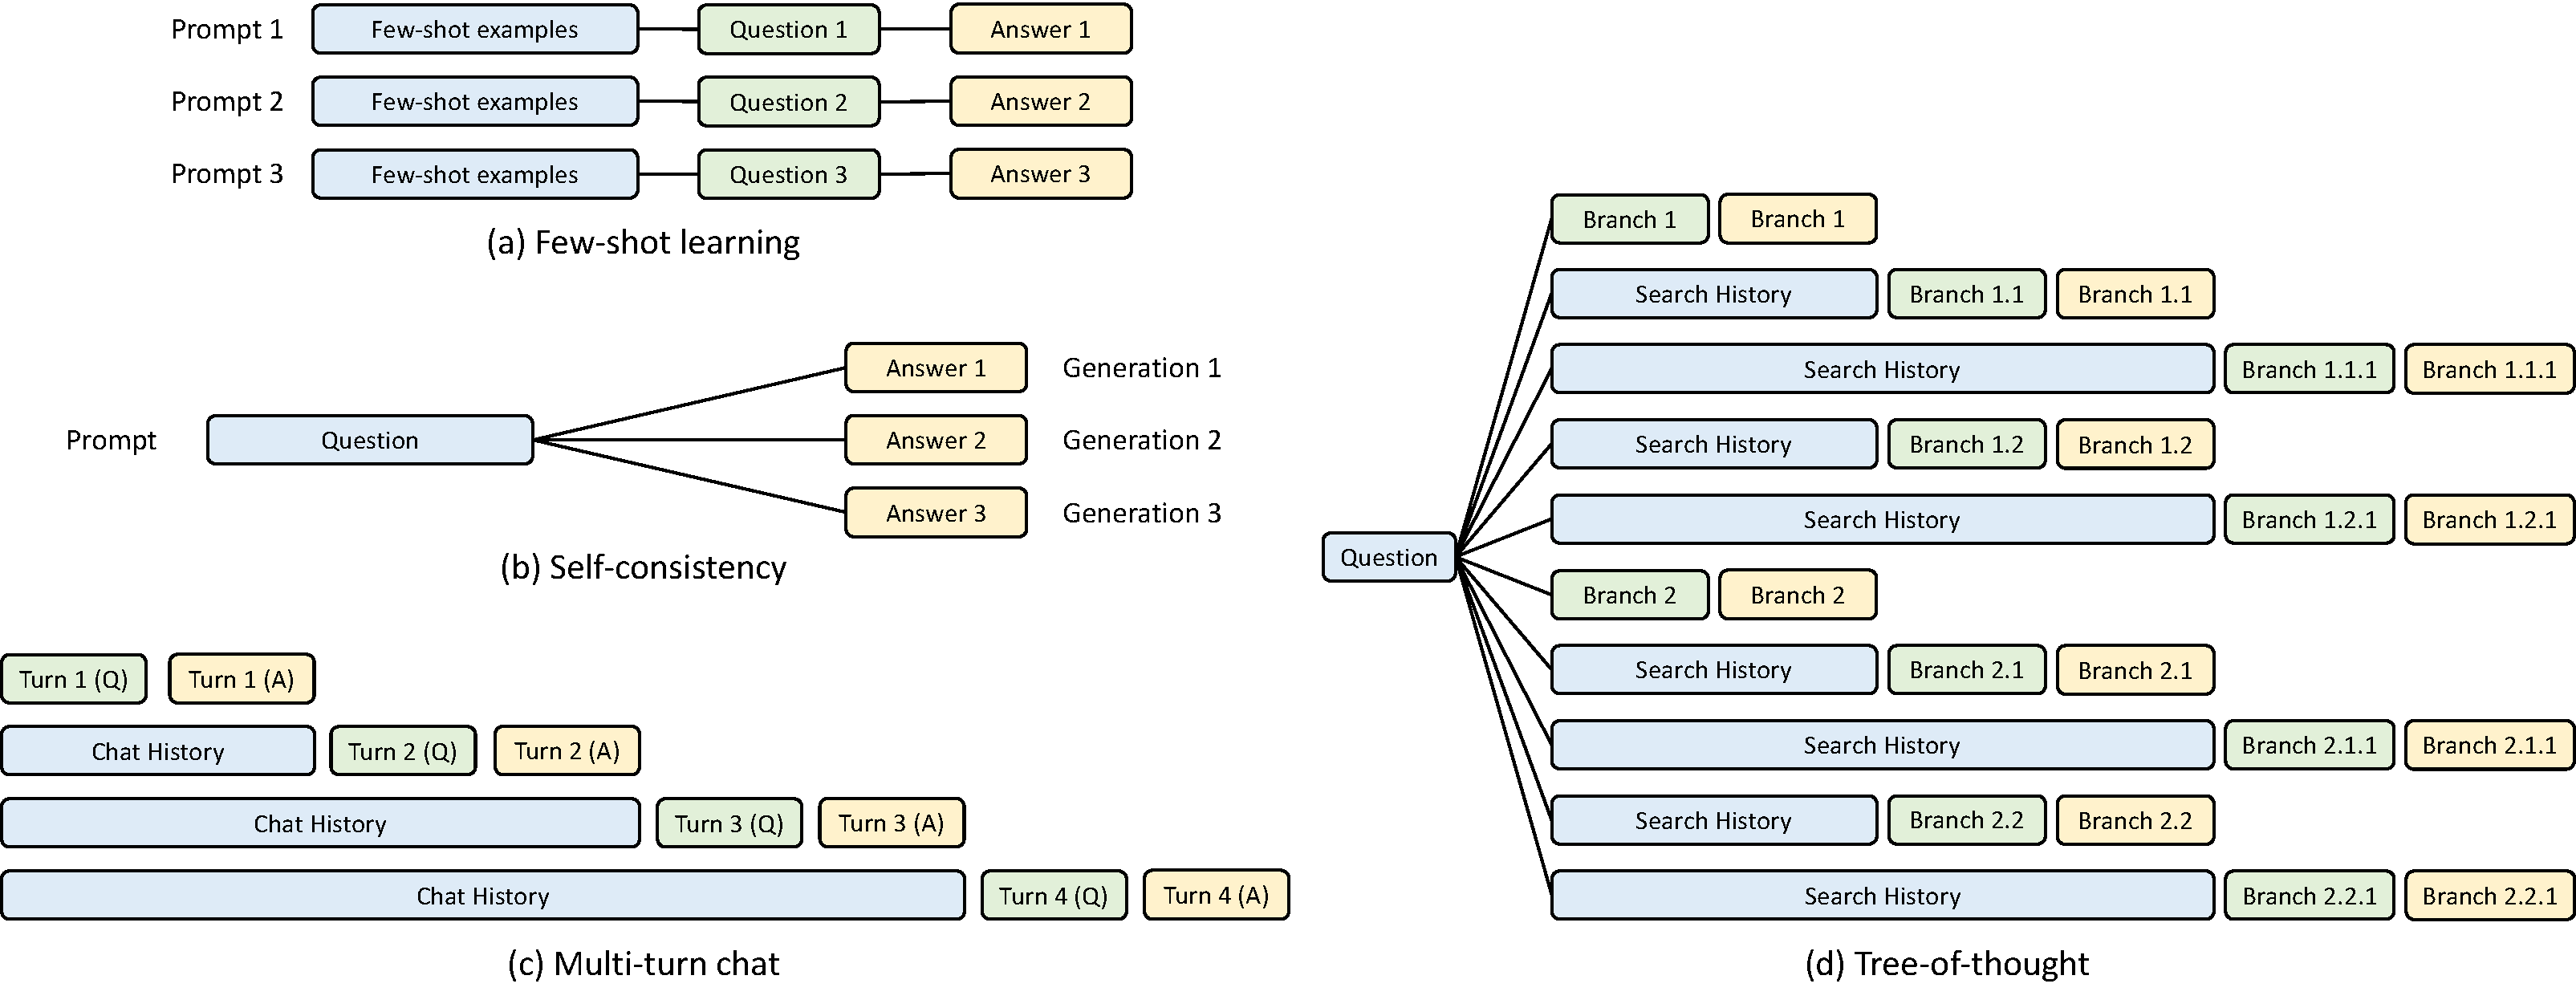
\includegraphics[width=\linewidth]{figures/example_sharing.pdf}
\vspace{-1em}
\caption{KV cache sharing examples. Blue boxes represent shareable prompt parts, green boxes indicate non-shareable parts and yellow boxes mark non-shareable model outputs. Shareable elements include few-shot learning examples, questions in self-consistency~\cite{wang2022self}, chat history in multi-turn chat, and search history in tree-of-thought~\cite{yao2023tree}.}
\label{fig:example_sharing}
\vspace{-1.5em}
\end{figure}

\begin{algorithm}[t]
\caption{Cache-Aware Scheduling for RadixAttention with Continuous Batching.}\label{alg:cache_aware_scheduling}
\begin{algorithmic}
\Require The radix tree $T$, the memory pool $P$, the current running batch $B$, the waiting queue $Q$.
\Ensure Finished requests and updated system state.

\State \text{// Get all requests from the waiting queue}
\State $requests \leftarrow Q.\text{get\_all\_requests}()$

\State \text{// Search for the prefix matching for all waiting requests}
\For{$req \in requests$}
    \State $req.prefix\_node, req.prefix\_len \leftarrow$ $T.\text{match\_prefix}(req.input\_tokens)$
\EndFor

\State \text{// Sort the requests according to the matched prefix lenghts}
\State $requests.\text{sort}()$

\State \text{// Select requests for the next batch}
\State $available\_size \leftarrow T.\text{evictable\_size}() + P.\text{available\_size}()$
\State $current\_size \leftarrow 0$
\State $new\_batch \leftarrow []$

\For{$req \in requests$}
    \If{$req.\text{size}() + current\_size < available\_size$}
        \State $new\_batch.\text{append}(req)$
        \State $delta \leftarrow T.\text{increase\_ref\_counter}(req.prefix\_node)$
        \State $available\_size \leftarrow available\_size + delta$
    \EndIf
\EndFor
\State $Q.\text{remove\_requests}(new\_batch)$

\State \text{// Insert requests into the current running batch}
\State $B.\text{merge}(new\_batch)$

\State \text{// Allocate new memory and do eviction if necessary}
\State $needed\_size \leftarrow B.\text{needed\_size}()$
\State $success, buffer \leftarrow P.\text{alloc}(needed\_size)$
\If{not $success$}
    \State $T.\text{evict}(needed\_size)$
    \State $success, buffer \leftarrow P.\text{alloc}(needed\_size)$
\EndIf

\State $B.\text{run}(buffer)$

\State \text{// Process finished requests}
\State $finished\_requests \leftarrow B.\text{drop\_finished\_requests}()$
\For{$req \in finished\_requests$}
    \State $T.\text{decrease\_ref\_counter}(req.prefix\_node)$
    \State $T.\text{insert}(req)$
\EndFor

\State \textbf{return} $finished\_requests$
\end{algorithmic}
\end{algorithm}


\subsection{Pseudocode for Cache-Aware Scheduling}
\label{subsec:pseudocode_cache_aware_scheduling}

\autoref{alg:cache_aware_scheduling} shows the pseudocode of cache-aware scheduling for RadixAttention with continuous batching.


\subsection{Proof of the \autoref{thm:optimal} }
\label{subsec:schedule_proof}

\optimal*
\begin{proof}
First, we show that the depth-first search (DFS) order achieves an optimal cache hit rate.
Let \( R \) denote the set of requests in the batch, and \( T \) denote the radix tree built from \( R \).
For each edge \( e \) of \( T \), the KV cache associated with \( e \) needs to be computed at least once.
Let \( |e| \) denote the size of the KV cache associated with \( e \).
Let \( C \) denote the computational complexity of the KV cache for \( R \).
We obtain the lower bound
\[
C \geq \sum_{e \in \text{edges}(T)} |e|.
\]

Consider we visit the radix tree \( T \) in DFS order.
For each edge \( e \) of \( T \), the first time we compute the KV cache associated with \( e \), we will then compute the whole subtree of \( e \).
During the computation of the subtree of \( e \), the edge \( e \) will be continuously hit, so no additional computation will happen. After finishing the computation for the subtree rooted at \( e \), the edge \( e \) will not be visited again.
Notice that, with a cache size \(\geq\) the maximum request length, which equals the longest path in the radix tree \( T \), edge \( e \) will not be evicted during the computation of its subtree, since the common prefix including \( e \) of the subtree will be continuously hit.
Therefore, the KV cache associated with each edge \( e \) will be computed only once. Thus, we achieve the lower bound
\[
C = \sum_{e \in \text{edges}(T)} |e|.
\]

The cache hit rate, defined as
\[
\frac{\sum_{r\in R}\text{number of cached prefill tokens in $r$}}{\sum_{r\in R}\text{number of prefill tokens in $r$}},
\]
equals \(1 - \frac{C}{\sum_{r\in R}\text{number of prefill tokens}}\), reaches its upper bound, delivering optimality.

Next, we show that the longest-shared-prefix-first order is equivalent to a DFS order by induction.
\begin{itemize}
    \item (Base) In the beginning, since there is nothing cached, a random request that corresponds to a node $x$ in $T$ will be processed. All requests that correspond to the nodes $\{v_1, ..., v_n\}$ on the path from the root to $x$ do not need a recomputation. The computation complexity for requests corresponding to the nodes $\{v_1,..., v_n, x\}$ is aligned with a valid DFS. The path from the root to $x$ is cached.

    \item (Induction) Assume we just visited a node $y$ in $T$, and the visited nodes align with a DFS order.
    Let $P$ denote the path from the root to $y$.
    Then each node that has not been visited has the lowest common ancestor with the visited nodes on $P$.
    Since nodes on $P$ are cached, a node $z$ that has not been visited with the lowest common ancestor on $P$ will have the longest shared prefix.
    The longest-shared-prefix-first order will select $z$, which is a valid DFS order. The path from the root to $z$ will be cached because it is the most recent.
\end{itemize}
\end{proof}

In the online case, the DFS order will be disrupted, but the longest shared prefix schedule still approximates the DFS behavior on the augmented part of the implied radix tree. We show this by considering the step of adding a new batch of requests.

Let \( T \) denote the part of the radix tree that has been visited so far, and \( T' \) denote the whole new radix tree after adding the new batch of requests. Let \( C \) denote the set of cached nodes in \( T \). Let \( \text{longest}(C) \) denote the node in \( C \) that has the longest path from the root and has a subtree in \( T' \) that has not been fully visited.

The longest shared prefix schedule will then process the subtree in $T'$ rooted at \( \text{longest}(C) \) in a DFS order. During this process, eviction could occur, and the remaining cached nodes from \( C \) become \( C^{(1)} \subseteq C \). A DFS will then occur for the subtree in $T'$ rooted at \( \text{longest}(C^{(1)}) \).

Similarly, we will have \( C^{(2)}, \ldots, C^{(k)} \), until \( C^{(k)} \) contains only one leaf node in \( C^{(k)} \) that has its subtree in $T'$ not fully visited. At this point, we have reached a valid DFS state. The remaining part of $T'$ will be visited in DFS order as described in the proof of \autoref{thm:optimal}.






\subsection{Data-Parallel Distributed RadixAttention}
\label{subsec:distributed_radix_attention}
To adapt the RadixAttention for distributed settings with multiple replica workers (i.e., data parallelism), we developed a mechanism wherein each worker maintains its own sub-tree, while the router oversees a meta-tree. 
This meta-tree acts as a trie that tracks all sub-trees and their associated devices. Upon the arrival of a new batch of requests at the router, prefix matching is executed on the meta-tree. We implement various policies based on each request's affinity—measured by the length of the shared prefix with specific workers and other requests in the same group—to make efficient dispatch decisions that minimize redundant computations.
Each time new requests are processed, both the router and workers independently update their respective trees. Should an eviction occur at a worker node, it commits this eviction to a queue, which the router then processes to update the meta-tree during periods of low activity.
We benchmarked this distributed configuration using four workers and the MMLU dataset, observing that it achieves linear scaling and an optimal cache hit rate with minimal overhead from this weakly consistent distributed cache design.
There exists a trade-off between maximizing data locality and parallel processing efficiency. Exploring advanced scheduling policies to optimize this trade-off is designated as an area for future research.
In addition, concurrent work from Preble~\cite{srivatsa2024preble} studies data-parallel scheduling based on an early version of SGLang.


\section{Additional Details on Compressed Finite State Machine}
\label{sec:additional_fsm}

This section discusses the background and implementation details of the compressed finite state machine for faster constrained decoding. We aim for LLMs to follow a regular expression (regex), which offers greater expressiveness and can be used to represent common formats such as JSON schemas. To achieve this, we convert the regex into a Finite State Machine (FSM) to guide the generation process during decoding~\cite{willard2023efficient}. An FSM is essentially a graph with nodes (states) and edges (transitions with strings/characters). Starting from an initial state, each transition appends the string on the edge to move to the next state, using a set of final states to conclude the process. This mechanism guides an LLM's decoding, filtering out invalid tokens based on the FSM's current state transitions, as illustrated in ~\autoref{fig:fsm_demo}. The decoding might involve multiple transitions in the FSM until reaching a final state.


\begin{figure}[ht]
    \centering
    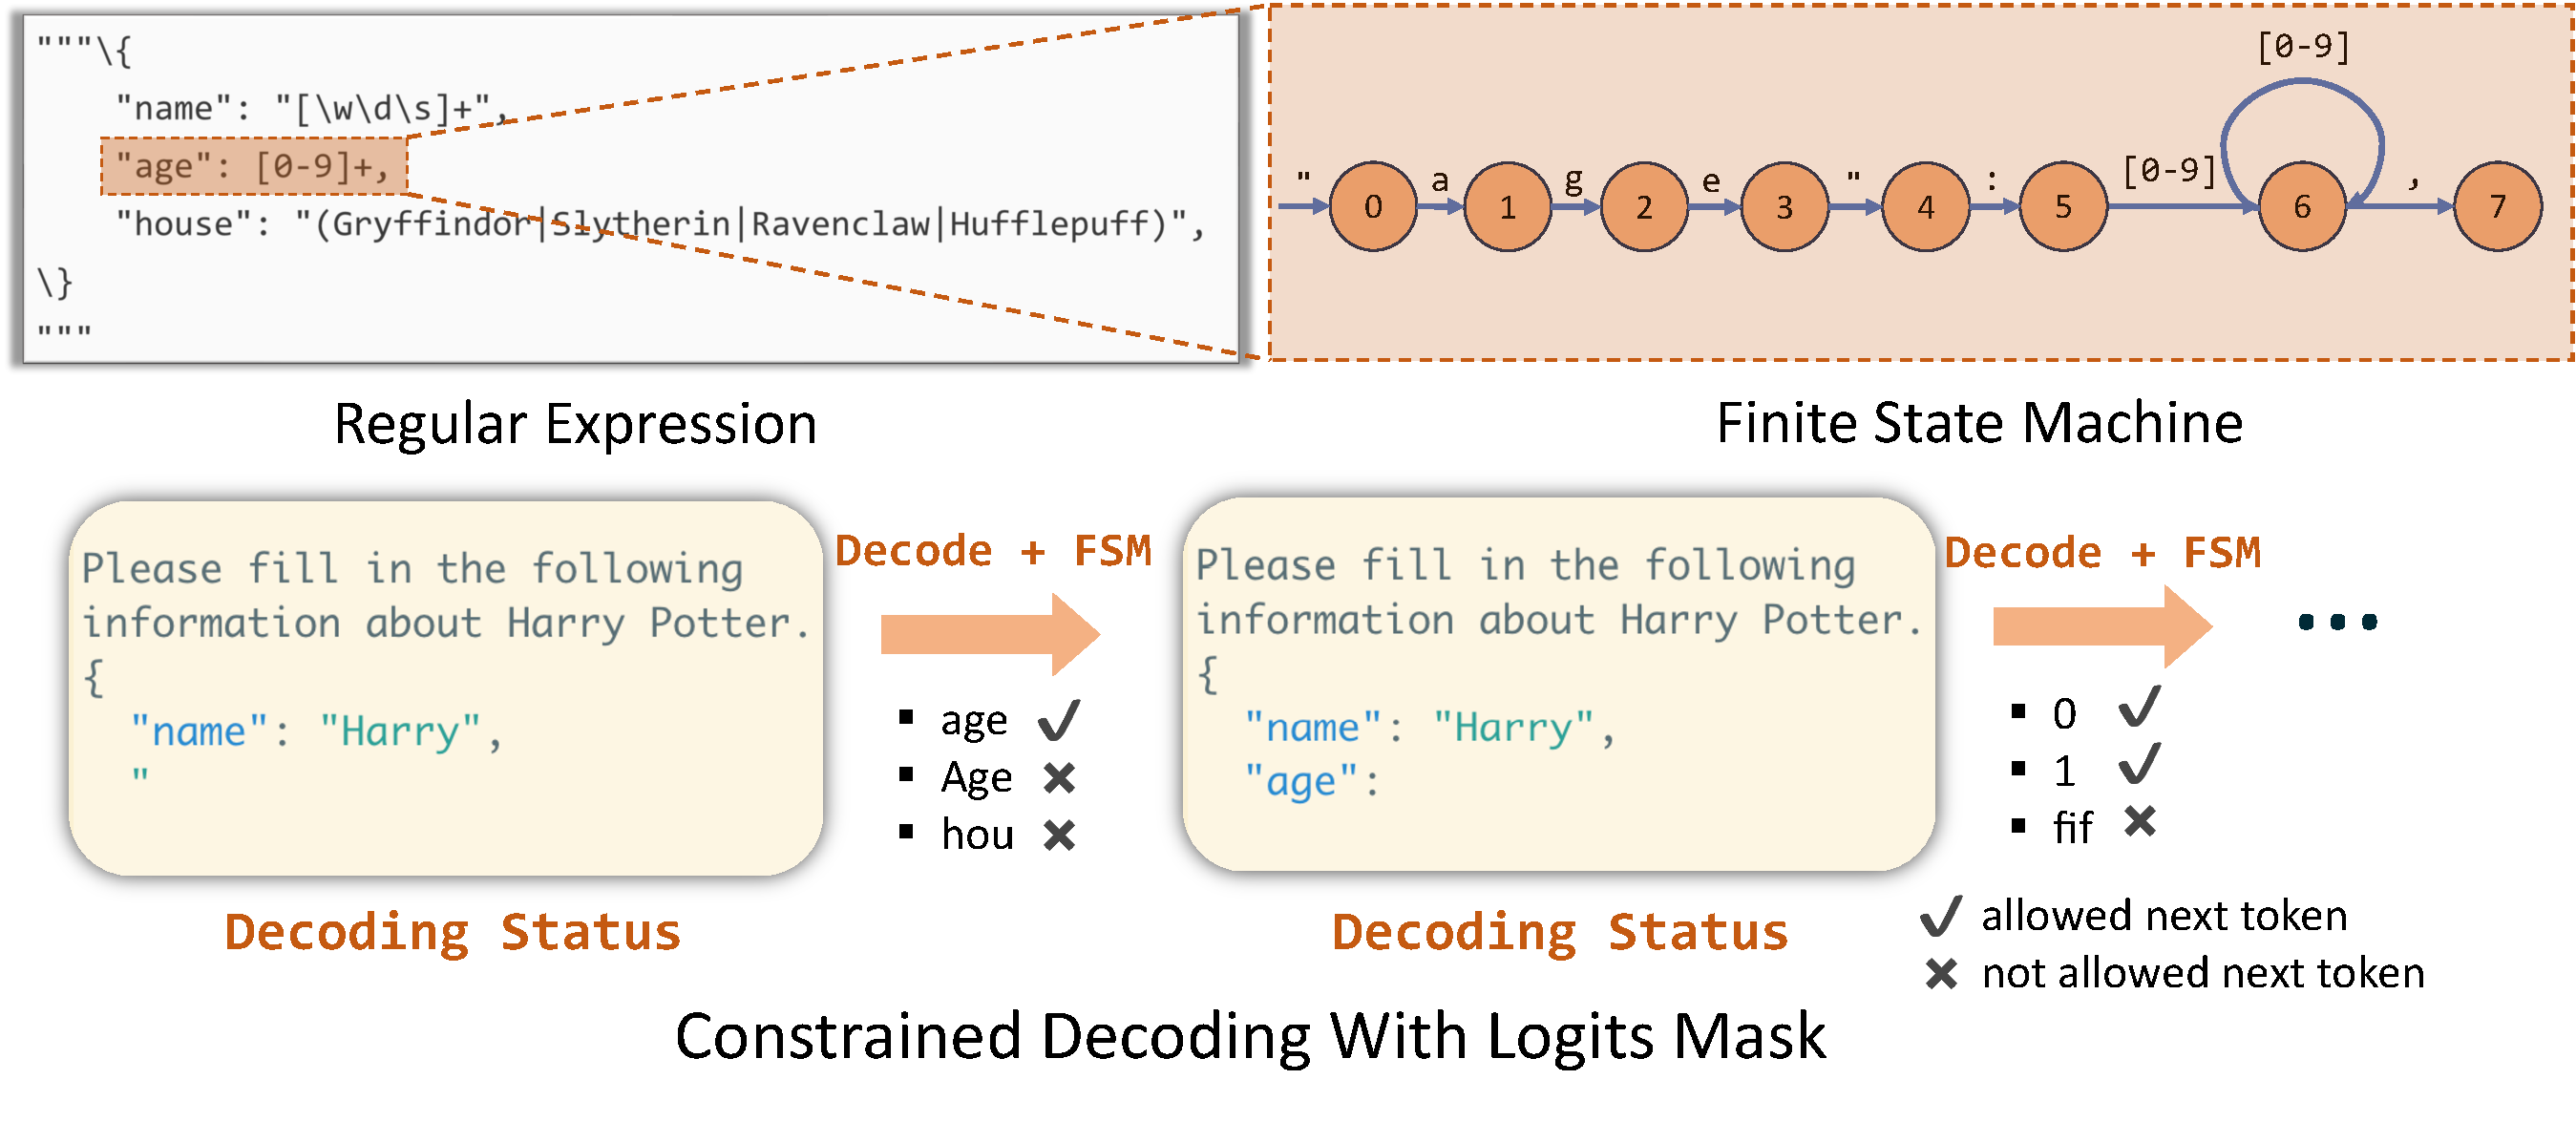
\includegraphics[width=\linewidth]{figures/fsm_demo.pdf}
    \vspace{-2em}
    \caption{Example of how regex is converted into FSM and how FSM guides the decoding process.}
    \vspace{-0.5em}
    \label{fig:fsm_demo}
\end{figure}

The challenge of constrained decoding arises from the fact that constraints are often expressed in natural language formats, i.e., regex is depicted by characters/strings, while LLMs are designed to interpret and process these as tokens. This creates a complex scenario since the mapping between strings and tokens is intricate and lacks a one-to-one correspondence ~\cite{kuchnik2023validating}.

This section is derived from an earlier blog post\footnote{\url{https://lmsys.org/blog/2024-02-05-compressed-fsm/}}. Readers are also encouraged to read the blog post for additional background and easier understanding.

\subsection{Implementation Details of Compressed Finite State Machine}

To simplify the construction of Compressed FSM, we build the original FSM on characters/strings instead of on tokens. We formally define the concepts of singular transition edge and compressed edge as follows:


\begin{itemize}
    \item Singular transition edge: A edge is a singular transition edge if 1) its source node has only one successor node, and 2) there is only one acceptable character/string on it.
    \item Compressed edge: An edge compressed by several consecutively adjacent edges $(e_0, e_1, \ldots, e_k)$ if and only if $e_1, \ldots, e_k$ are singular transition edges. The text of the compressed edge is the concatenation of the texts of $e_0, e_1, \ldots, e_k$.
\end{itemize}


Starting from an FSM based on characters, we recursively merge singular transition edges into their preceding ones until further compression is unfeasible, resulting in a Compressed FSM. This approach speeds up the decoding process, as demonstrated by \lang's runtime efficiency with the Compressed FSM, shown in ~\autoref{fig:compressed_fsm}.

\begin{figure}[ht]
    \centering
    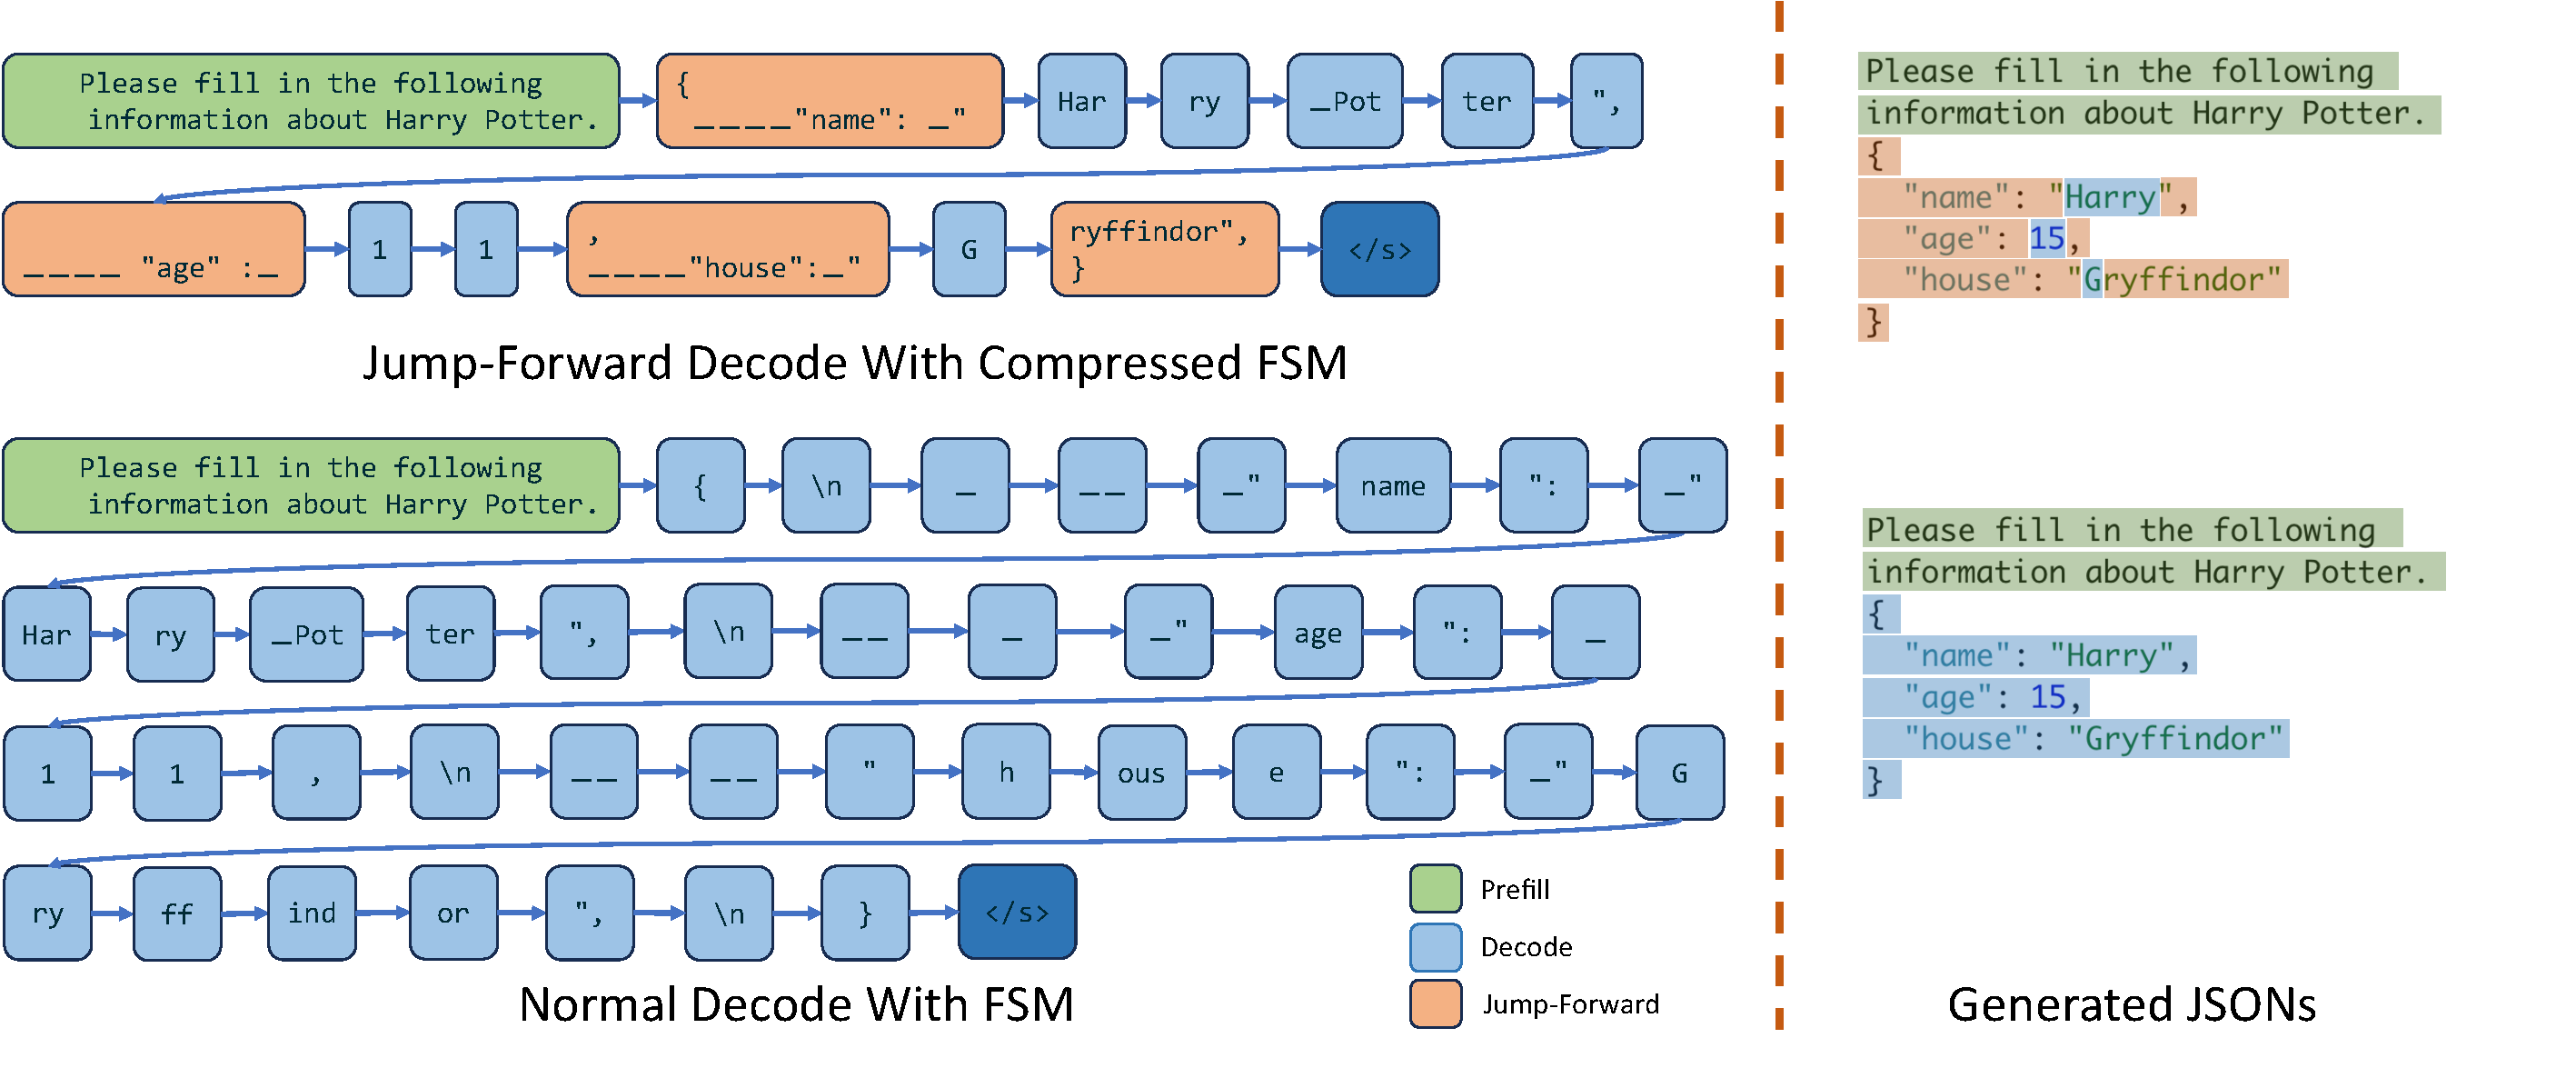
\includegraphics[width=\linewidth]{figures/compressed_fsm.pdf}
    \vspace{-2em}
    \caption{Comparison of decoding using Compressed FSM versus normal FSM: The left subfigure depicts the decoding process per forward pass, while the right subfigure explains the origins of various result components.}
    \vspace{-1.5em}
    \label{fig:compressed_fsm}
\end{figure}

\subsection{Handling Tokenization Artifacts with Retokenization}

When a new token is generated, we get the token's string and search all the outgoing edges of the current state find the one that starts with the just decoded string, and then move forward. However, when the transition edge is a well-compressed one and contains a very long string, we may anticipate the next rounds' decoded strings as well. This is where the acceleration happens and we call this process \textit{Jump Forward}. However, we still need to convert the string into tokens for the next decoding phases and it is not straightforward due to the LLM's specific pretraining and tokenization method; direct partitioning might alter the intended meaning~\cite{Tran-Thien_2024}. For example, the compressed text in \autoref{fig:example_first_program}'s regex is \texttt{\{"summary":\ "}, which can only be tokenized as \texttt{\{"}, \texttt{summary}, \texttt{":} and \texttt{\_"} according to the tokenizer instead of partition them randomly such as \texttt{\{"}, \texttt{summa}, \texttt{ry}, and \texttt{":\_"}. To address this issue, we use the original tokenizer to retokenize all the previous text as well as the text of the compressed edge, ensuring alignment with the original input format of LLMs. And it only brings minor retokenization overhead.

\subsection{Future Extension: Addressing Distorted Probability}

The challenge caused by the gap between strings and tokens also brings the problem of skewed probability distribution~\cite{Tran-Thien_2024}. For example, in \autoref{fig:example_first_program}, the regex \texttt{"[ABCD][+-]?"} suggests grades from \texttt{A+} to \texttt{D-}, but if replaced with broader terms like \texttt{Excellent|Above Average|Fair|Below Average}, the runtime may inaccurately map an \texttt{A} to \texttt{Above Average} due to the term \texttt{Above Average} is on a compressed transition, misrepresenting the grade hierarchy. This occurs because the LLM doesn't recognize the specific range of choices, leading to inappropriate token sequences. Computing accurate probabilities for each choice requires summing the probabilities of all token sequences that result in each choice, which complicates decoding and adds overhead. One workaround is to include the choices or the regex directly in the prefill prompt, guiding the LLM to be aware of its choices and output the decision in proper token sequences. However, this approach doesn't solve the underlying issue of distorted probabilities, highlighting the need for further research to improve the compressed FSM's accuracy.




\section{Additional Experimental Setups and Results}
\label{sec:additional_experimental_results}

\textbf{Additional experimental setups.}
\autoref{fig:exp_llama_7b_throughput} and \autoref{fig:exp_llama_7b_latency} are obtained by running Llama-7B on a single A10G (24GB) GPU.
\autoref{fig:exp_mixtral_8x7b_throughput} are obtained by running Mixtral-8x7B on 8 A10G (24GB) GPUs with tensor parallelism.
\autoref{fig:exp_hit_rate_vs_perf}(c) is obtained by running Llama-7B on a single A10G (24GB) GPU.
\autoref{fig:exp_llama_70b_throughput} are obtained by running Llama-70B on 4 A100G (80GB) GPUs with tensor parallelism.
\autoref{tab:e2e_multi_modal} are obtained by running LLaVA-v1.5-7B on a single A10G (24GB) GPU and running LLaVA-Next-34B on a single A100G (80GB) GPU.
Each bar in the benchmark figures takes several minutes to an hour to run.

\textbf{Additional experimental results.}
\autoref{fig:exp_cache_hit_rate} shows the achieved and optimal cache hit rates on the benchmarks listed in \autoref{fig:exp_llama_7b_throughput}.
\autoref{fig:exp_llama_70b_throughput} shows the throughput on Llama-2-70B with tensor parallelism.

\begin{figure}[t]
\centering
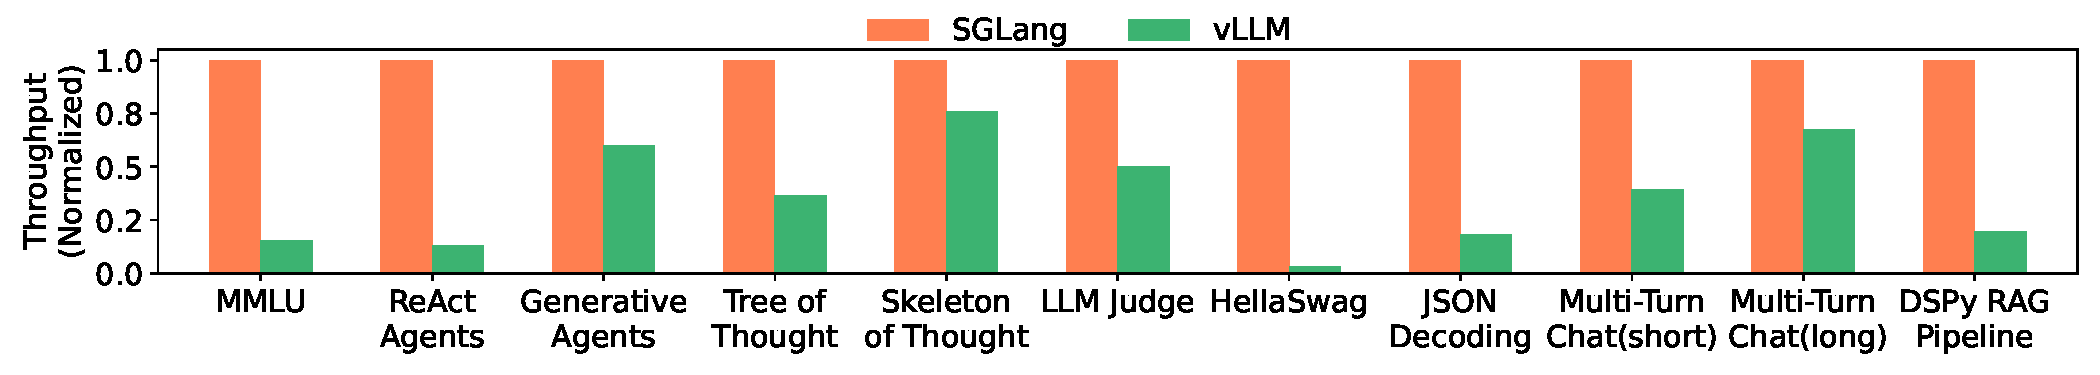
\includegraphics[width=\linewidth]{figures/e2e_throughput_llama_70b.pdf}
\vspace{-2em}
\caption{Normalized throughput on Llama-2-70B models with tensor parallelism. Higher is better.}
\label{fig:exp_llama_70b_throughput}
\end{figure}

\begin{figure}[t]
\centering
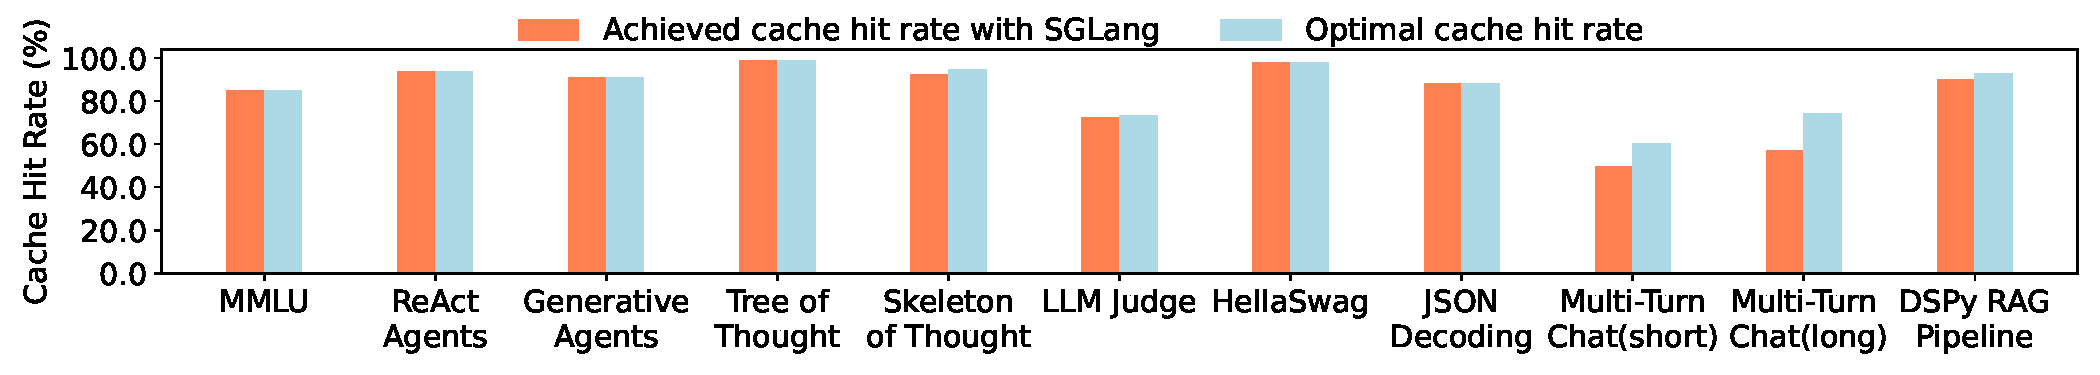
\includegraphics[width=\linewidth]{figures/optimal_cache_hit_rate.pdf}
\vspace{-2em}
\caption{Achieved cache hit rate and optimal cache hit rate on various benchmarks.}
\label{fig:exp_cache_hit_rate}
\end{figure}



\begin{figure}[t]
    \centering
    \begin{subfigure}{0.47\textwidth}
        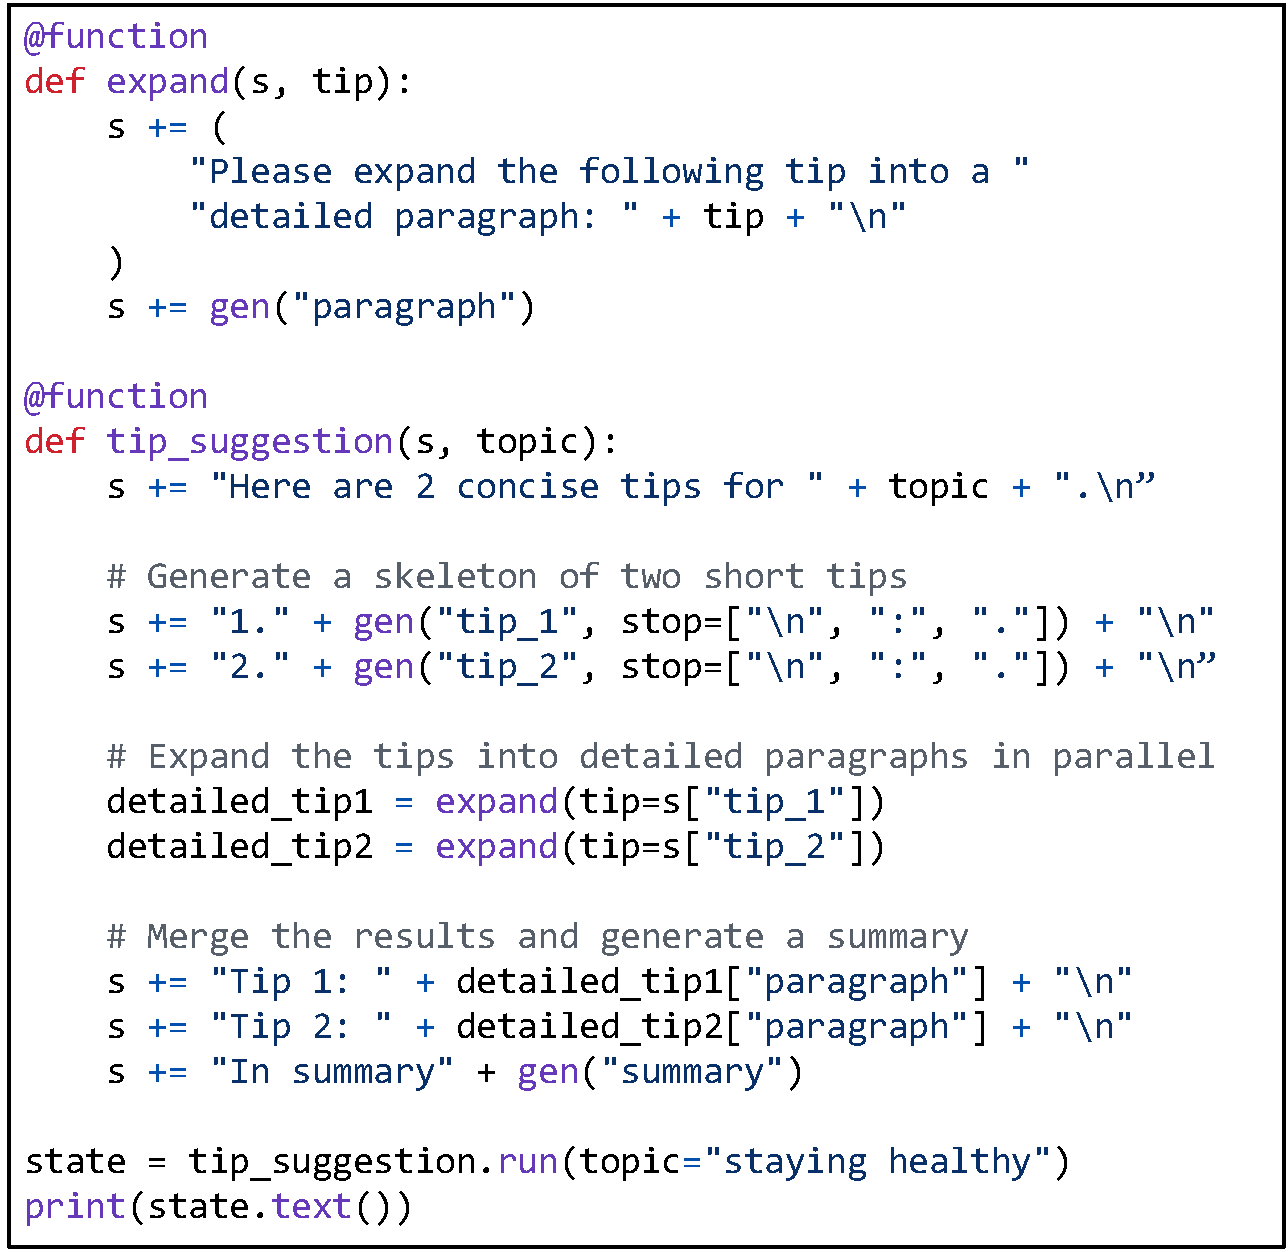
\includegraphics[width=\linewidth]{figures/example_tip_suggestion.pdf}
        \caption{The \lang program for parallel tip suggestion with skeleton-of-thought prompting.}
        \label{fig:example_tip_suggestion}
    \end{subfigure}
    \hfill
    \begin{subfigure}{0.47\textwidth}
        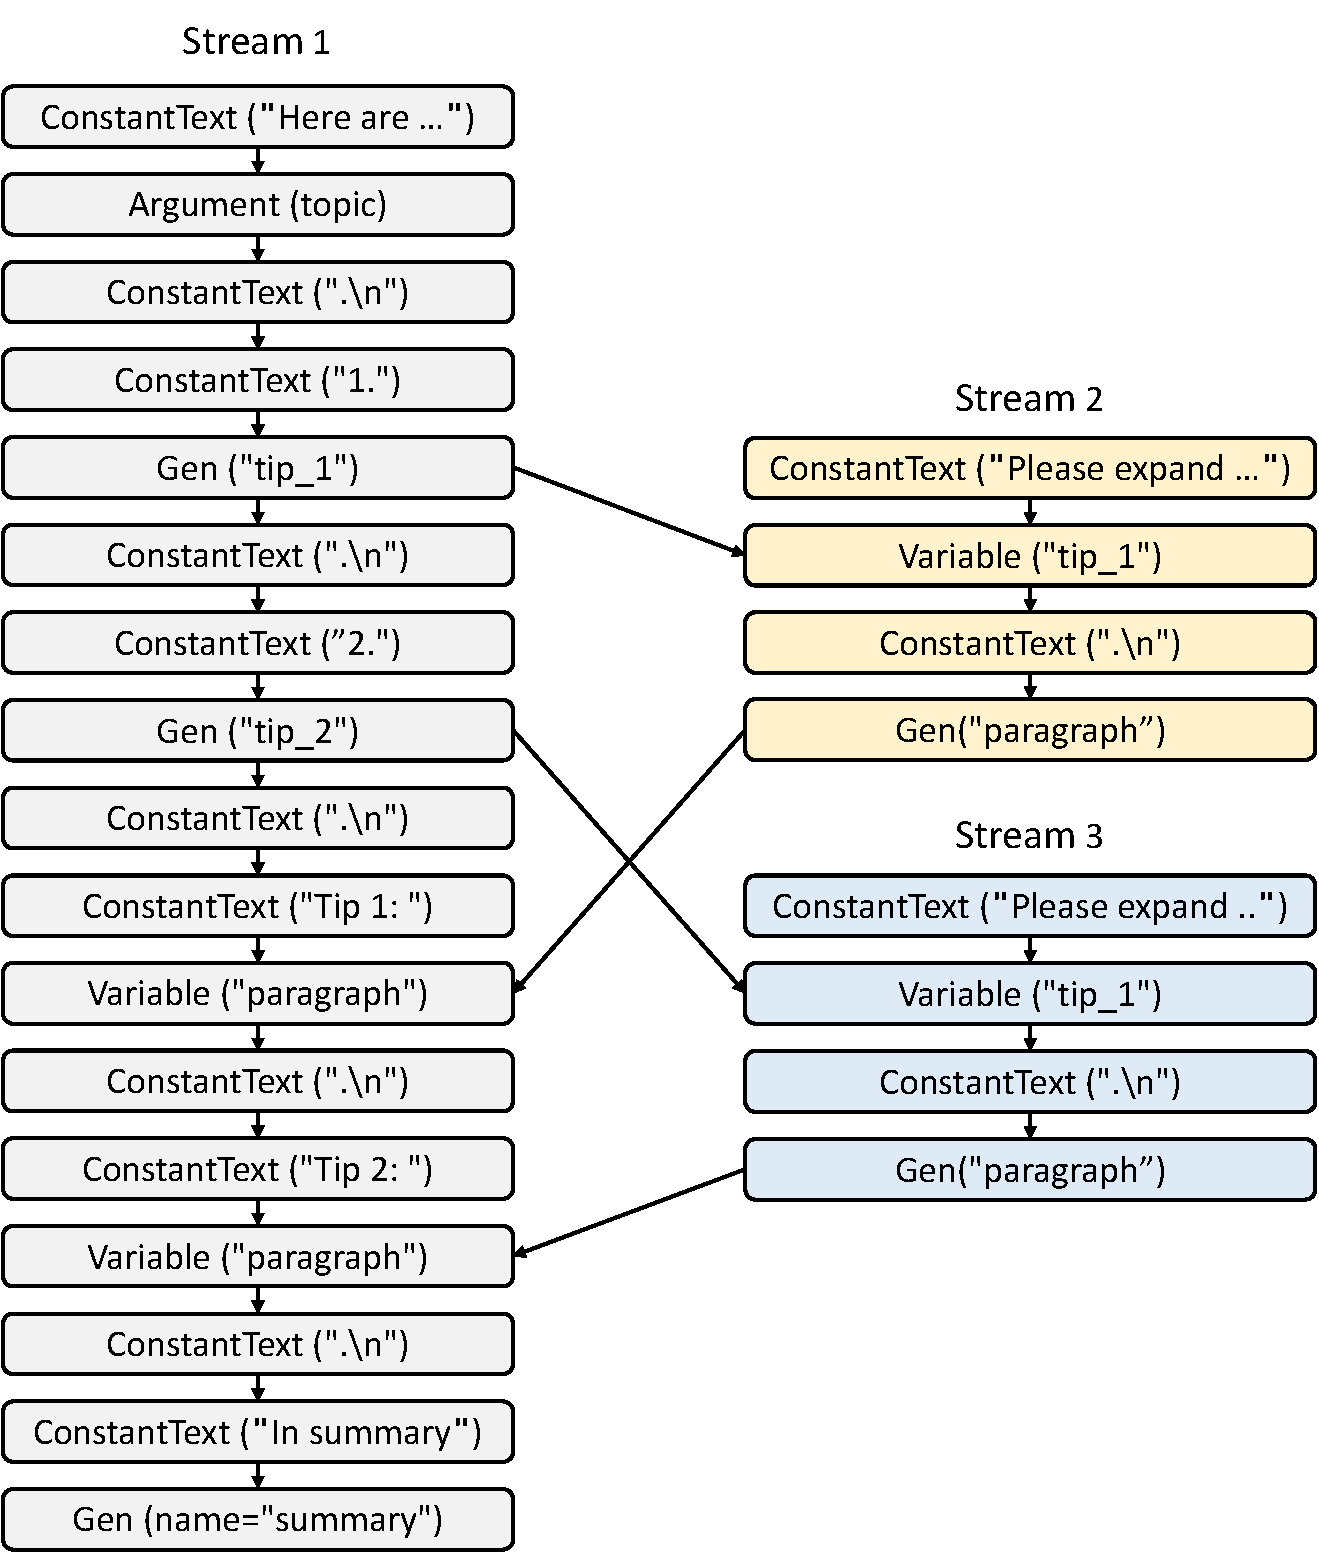
\includegraphics[width=\linewidth]{figures/example_dataflow_graph.pdf}
        \caption{A computational graph for the program in \autoref{fig:example_tip_suggestion}. The three streams correspond to three function calls.}
        \label{fig:example_dataflow_graph}
    \end{subfigure}
    \caption{An \lang program and its corresponding dataflow graph.}
\end{figure}


\section{Compiler Mode}
\label{sec:compiler_mode}
Besides the interpreter mode used in the main body of the paper, another way to run \lang programs is to compile them as computational graphs and execute them with a graph executor. This opens up opportunities for more compilation optimizations, as we can rewrite the graph and perform more static planning.

\subsection{Design and Implementation}

We designed an intermediate representation (IR) for \lang, which represents \lang program structures and operations as a computational graph. This graph includes nodes for primitive operators and edges for dependencies. See \autoref{fig:example_dataflow_graph} for the graph corresponding to the program in \autoref{fig:example_tip_suggestion}. In the program, each call to a decorated function or fork creates a new prompt state or a stream.

There are several types of nodes. Each operand of the operators \texttt{+=} and \texttt{+} in a \lang program is represented by an IR node. These include \texttt{ConstantText}, \texttt{Argument}, \texttt{Gen}, \texttt{Select}, \texttt{Variable}, \texttt{Fork}, \texttt{GetForkItem}, and \texttt{Join}. There are two types of dependencies: intra-stream dependency, where operations submitted into a stream using \texttt{+=} must be executed after all preceding operations in that stream, and inter-stream dependency, which occurs when one stream needs to fetch variable values from another stream, necessitating synchronization. Operations like fork manipulate multiple streams and thus introduce inter-stream dependencies.

To generate the graph, we use tracing to run the program with abstract arguments and construct the graph dynamically. This method is limited to programs without data-dependent control flow, a limitation we plan to address in future work. Once constructed, the graph can be executed through a graph executor, eliminating the need to reinterpret the original Python program. This results in benefits like graph rewriting optimizations, reduced runtime overhead, and program serialization. For execution, stream executors are launched for each data stream, dispatching IR nodes to the streams in topological order.


\subsection{A Case Study of Compiler Optimization: Code Movement for Improving Prefix Sharing}
We explore a compilation optimization for \lang IR: code movement for improving prefix sharing. We anticipate that more classical compiler techniques can also be applied, such as auto-tuning and instruction selection.

This optimization aims to improve prefix sharing by reordering nodes in the graph to increase the length of the constant prefix. It does not strictly preserve the original computation, classifying it as an aggressive optimization. For instance, changing the prompt from ``Here is a question + \{question\}. Please act as a math expert and solve the given question.'' to ``Please act as a math expert and solve the given question. Here is a question + \{question\}.'' results in a longer shareable prefix. This optimization is interesting because traditional program analysis cannot achieve it due to the presence of natural language instructions in \lang. Instead, we prompt GPT-4 to reorder graph nodes. We write a prompt with several examples to teach GPT-4 the concepts of \lang IR, and we find that GPT-4 can successfully apply this optimization for some simple \lang programs.

We evaluate the effectiveness of this optimization. We collect 20 prompt templates from the internet and implement them in \lang. We utilize 5 of these templates as few-shot training examples and the remaining 15 as test cases. Our evaluation shows that, for 12 out of the 15 templates, GPT-4 successfully reorders the graph nodes without altering the semantics, as confirmed by manual inspection of the modified prompts. On average, this optimization results in a 60-token increase in the shareable prefix length, showcasing GPT-4's effectiveness. Failures in creating optimized prompt order come from an incorrect understanding of the semantic meaning behind the graph nodes. It is too aggressive and puts all constants upfront even when such ordering changes the original semantics. This case study aims to explore the use of GPT-4 for compiler optimizations. More work is needed to make these kinds of optimizations reliable in the future.


